\documentclass[]{article} 
\usepackage{pgfplots} 
\usepgfplotslibrary{external} 
\tikzexternalize 
\usepgfplotslibrary{fillbetween}
\usepackage{tikz} 
\usepackage{amsmath} 
\usepackage{pgfplots} 
\usetikzlibrary{calc} 
\pgfplotsset{compat = newest,every x tick label/.append style={font=\scriptsize,color = white},every y tick label/.append style={font=\scriptsize,color = white}, every axis plot post/.style={line join=round}}

\begin{document} 
	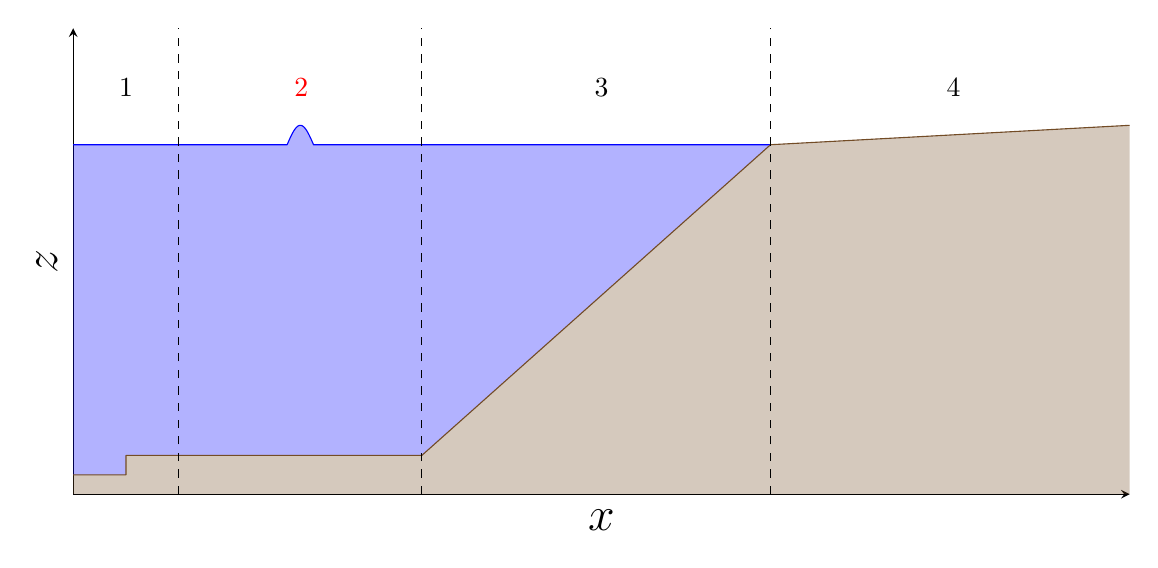
\begin{tikzpicture} 
	\begin{axis}[ 
	width = 0.7\textwidth,
	label style={font=\LARGE},
	axis lines=left, xtick=\empty,
	ytick={-1},
	clip mode=individual,
	xmin=0, 
	xmax=1, 
	width = 15cm,
	height = 7.5cm,
	ymin = -0.1, 
	ymax = 1.1,
	xlabel=$x$, 
	ylabel=$z$ ]
	
	\addplot[name path=g,blue] coordinates{(0,0.8) (0.2025,0.8) 
		(0.20250000000000001, 0.80000000000000004)
		(0.20336206896551726, 0.80540595092119716)
		(0.2042241379310345, 0.81074852201055125)
		(0.20508620689655174, 0.81596507650679906)
		(0.20594827586206899, 0.82099445507801327)
		(0.20681034482758623, 0.82577769285885116)
		(0.20767241379310347, 0.83025871075968838)
		(0.20853448275862069, 0.83438497294267111)
		(0.20939655172413793, 0.83810810275638181)
		(0.21025862068965517, 0.84138444990784456)
		(0.21112068965517242, 0.84417560222230115)
		(0.21198275862068966, 0.84644883599083964)
		(0.2128448275862069, 0.84817749962596123)
		(0.21370689655172415, 0.84934132612707636)
		(0.21456896551724139, 0.84992667069255623)
		(0.21543103448275863, 0.84992667069255623)
		(0.21629310344827588, 0.84934132612707636)
		(0.21715517241379312, 0.84817749962596123)
		(0.21801724137931036, 0.84644883599083964)
		(0.2188793103448276, 0.84417560222230115)
		(0.21974137931034485, 0.84138444990784456)
		(0.22060344827586209, 0.83810810275638181)
		(0.22146551724137931, 0.83438497294267133)
		(0.22232758620689655, 0.83025871075968838)
		(0.22318965517241379, 0.82577769285885116)
		(0.22405172413793104, 0.82099445507801339)
		(0.22491379310344828, 0.81596507650679917)
		(0.22577586206896552, 0.81074852201055125)
		(0.22663793103448276, 0.80540595092119716)
		(0.22750000000000001, 0.80000000000000004)
		(0.2275,0.8) (0.66,0.8)};
	%\addplot [ blue] coordinates {(0,0.8) (0.025,0.8)};
	%\addplot [smooth, blue] coordinates {(0.025,0.8) (0.03166666666,0.75)  (0.05,0.8) (0.06666666666,0.85)  (0.075,0.8)};
	%\addplot [ blue] coordinates {(0.075,0.8) (0.66,0.8)};
	
    \path[name path=axis] (axis cs:0,-0.1) -- (axis cs:1,-0.1);
    
    \addplot[name path=f, brown!60!black] coordinates {(0,-0.05) (0.05,-0.05) (0.05,0) (0.33,0) (0.66,0.8) (1,0.85)};
    
    \addplot [
    thick,
    color=brown!60!black,
    fill=brown!60!black, 
    fill opacity=0.3
    ] fill between[of=f and axis];
    
    \addplot [
    thick,
    color=blue,
    fill=blue, 
    fill opacity=0.3
    ] fill between[of=g and f];
	
	
	\node[above] at (0.05,0.9) {1};
	\addplot [black,dashed] coordinates {(0.1,-0.1) (0.1,1.1)};
	
	\node[above] at (0.216,0.9) {\color{red}{2}};
	\addplot [black,dashed] coordinates {(0.33,-0.1) (0.33,1.1)};
	
	\node[above] at (0.5,0.9) {3};
	
	\addplot [black,dashed] coordinates {(0.66,-0.1) (0.66,1.1)};

	\node[above] at (0.8333,0.9) {4};
	
	\end{axis} 
	\end{tikzpicture} 
\end{document}